
\section{INTRODUCTION \& MOTIVATION}

(team part)

There are five sections in this template, please follow the sections and feel free to add sub-sections. 

In this section, you need to give an introduction of your team's project started with a couple of sentences that introduce your topic to your readers. You do not have to give too much detailed information, but you explain why this project is important.

You should also have a literature review about relevant publications in BibTex format, for example, citing AprilTags~\cite{Olson09icra}. You should stand on giant's shoulder and know what have been done in the past. Recent papers in ICRA, IROS, RSS, CVPR, ICCV, ECCV, and etc. in the past 5 years, or a survey/review paper will be very helpful.

This IEEE template provides authors with most of the formatting specifications needed for preparing electronic versions of their papers. All standard paper components have been specified for three reasons: (1) ease of use when formatting individual papers, (2) automatic compliance to electronic requirements that facilitate the concurrent or later production of electronic products, and (3) conformity of style throughout a conference proceedings. Margins, column widths, line spacing, and type styles are built-in; examples of the type styles are provided throughout this document and are identified in italic type, within parentheses, following the example. Some components, such as multi-leveled equations, graphics, and tables are not prescribed, although the various table text styles are provided. The formatter will need to create these components, incorporating the applicable criteria that follow.

\begin{figure}[t]
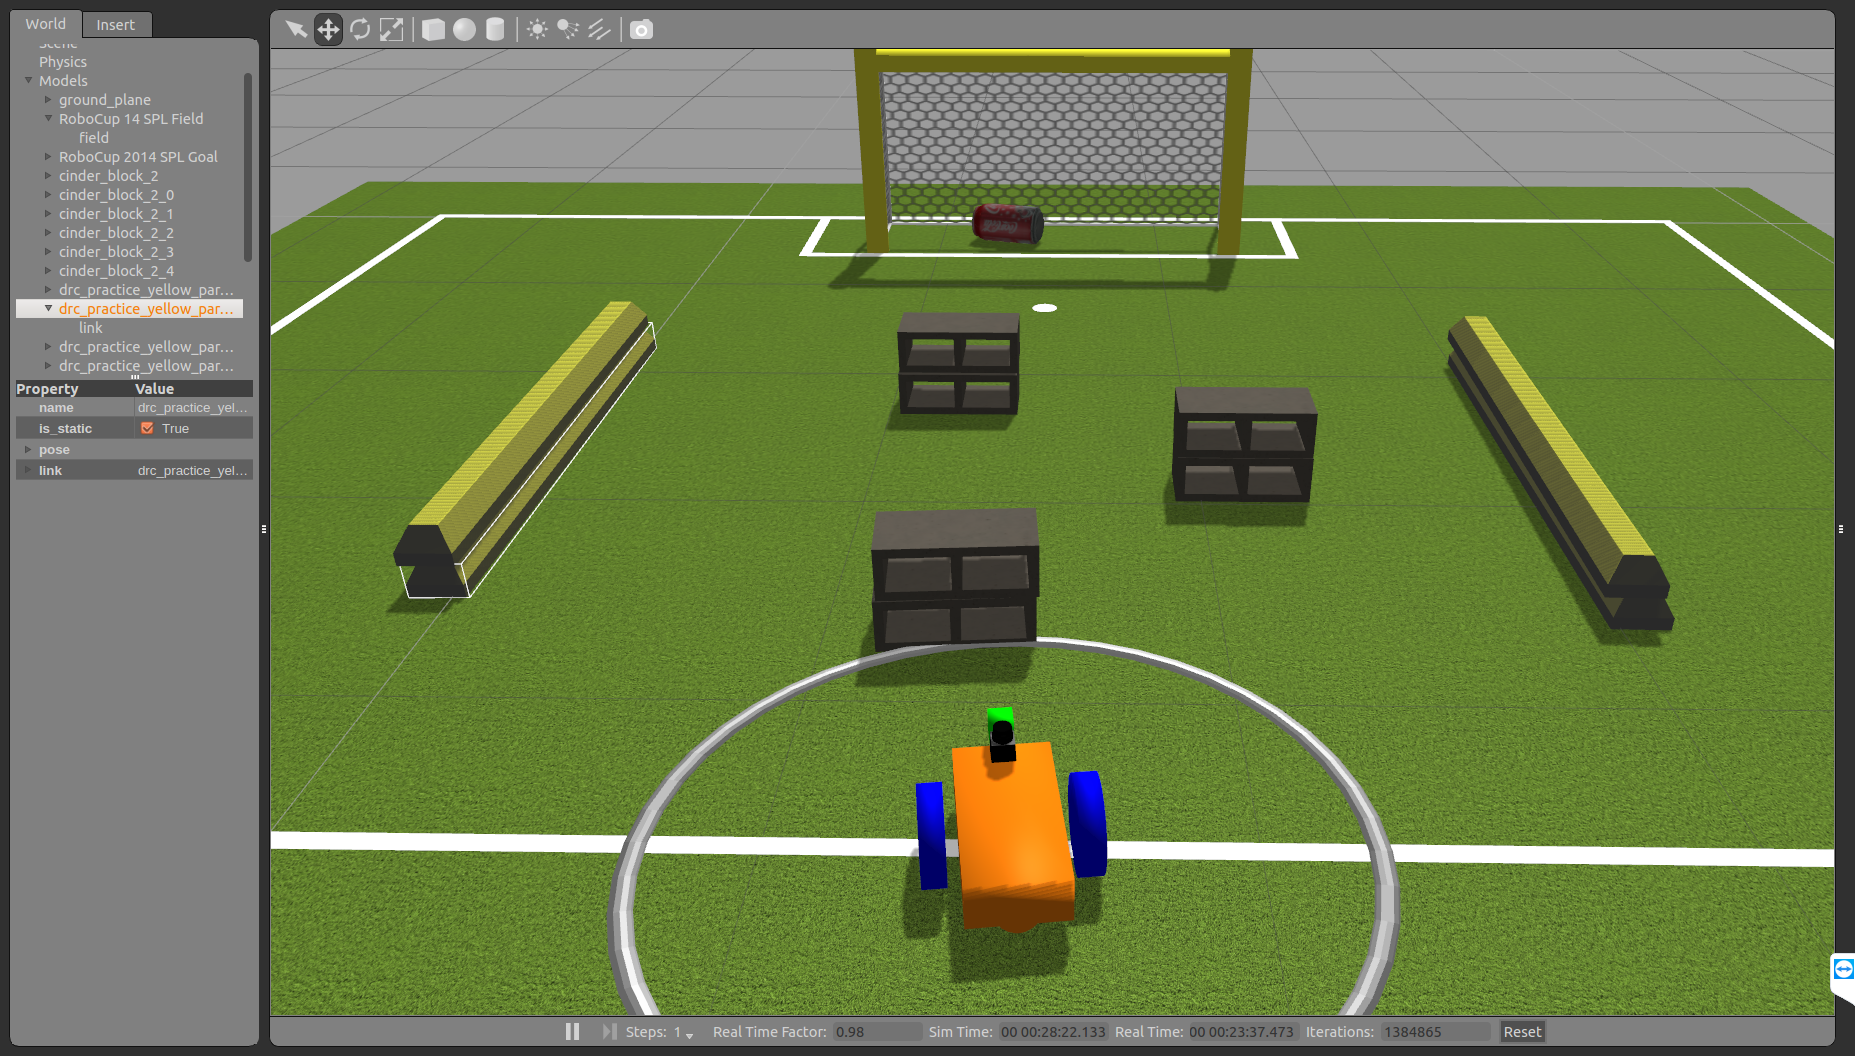
\includegraphics[width=0.95\columnwidth]{gazebo_view}
\centering
\caption{Teaser figure: this figure is the most important one in the paper. It gives your readers the first impression of this work. The teaser generally includes the overview of the proposed approach and the key contributions. It appears at the upper right of the first page.}
\end{figure}

\section{SYSTEM ARCHITECTURE \& EQUIPMENTS}

(team part)

\subsection{SYSTEM ARCHITECTURE}

This section explains the approaches in both hardware or software systems. You should explain here the key components/modules and they are working together (typically in a flowchart). Wherever possible, the methods and tasks to be performed should be outlined in logical sequence and explained in detail. Do not assume the reviewer will fill in the gaps in your logic. A ROS system diagram generated by rqt\_graph~\cite{rqt-graph} may be useful.

\subsection{EQUIPMENTS} 

You should list the hardware which is necessary in your project. Your project will only become For example, UR5 collaborative robotics arm in Fig.~\ref{figure:ur5}, MIT2.12 mobile manipulators in Fig.~\ref{figure:mit212mm}, and Intel Realsense SR300~\ref{figure:sr300} ....

\begin{figure}[!b]
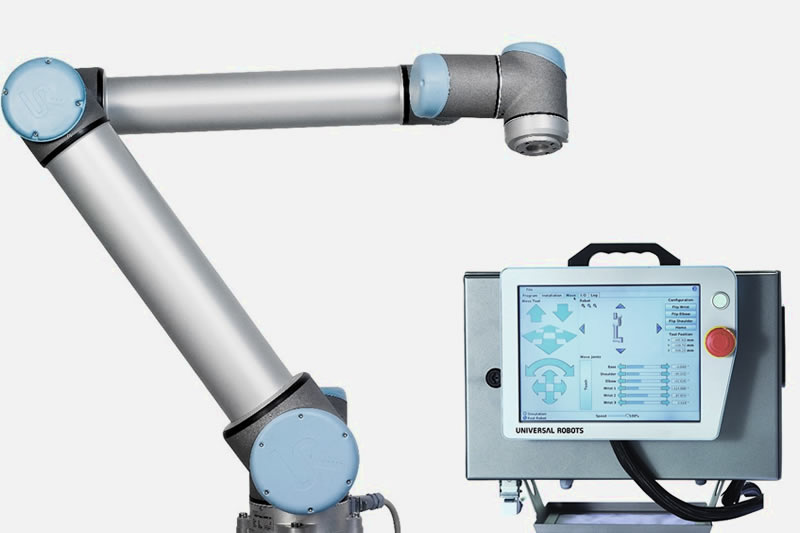
\includegraphics[width=0.7\columnwidth]{UR5}
\centering
\caption{UR5 robotic arm}
 \label{figure:ur5}
\end{figure}

\begin{figure}[h]
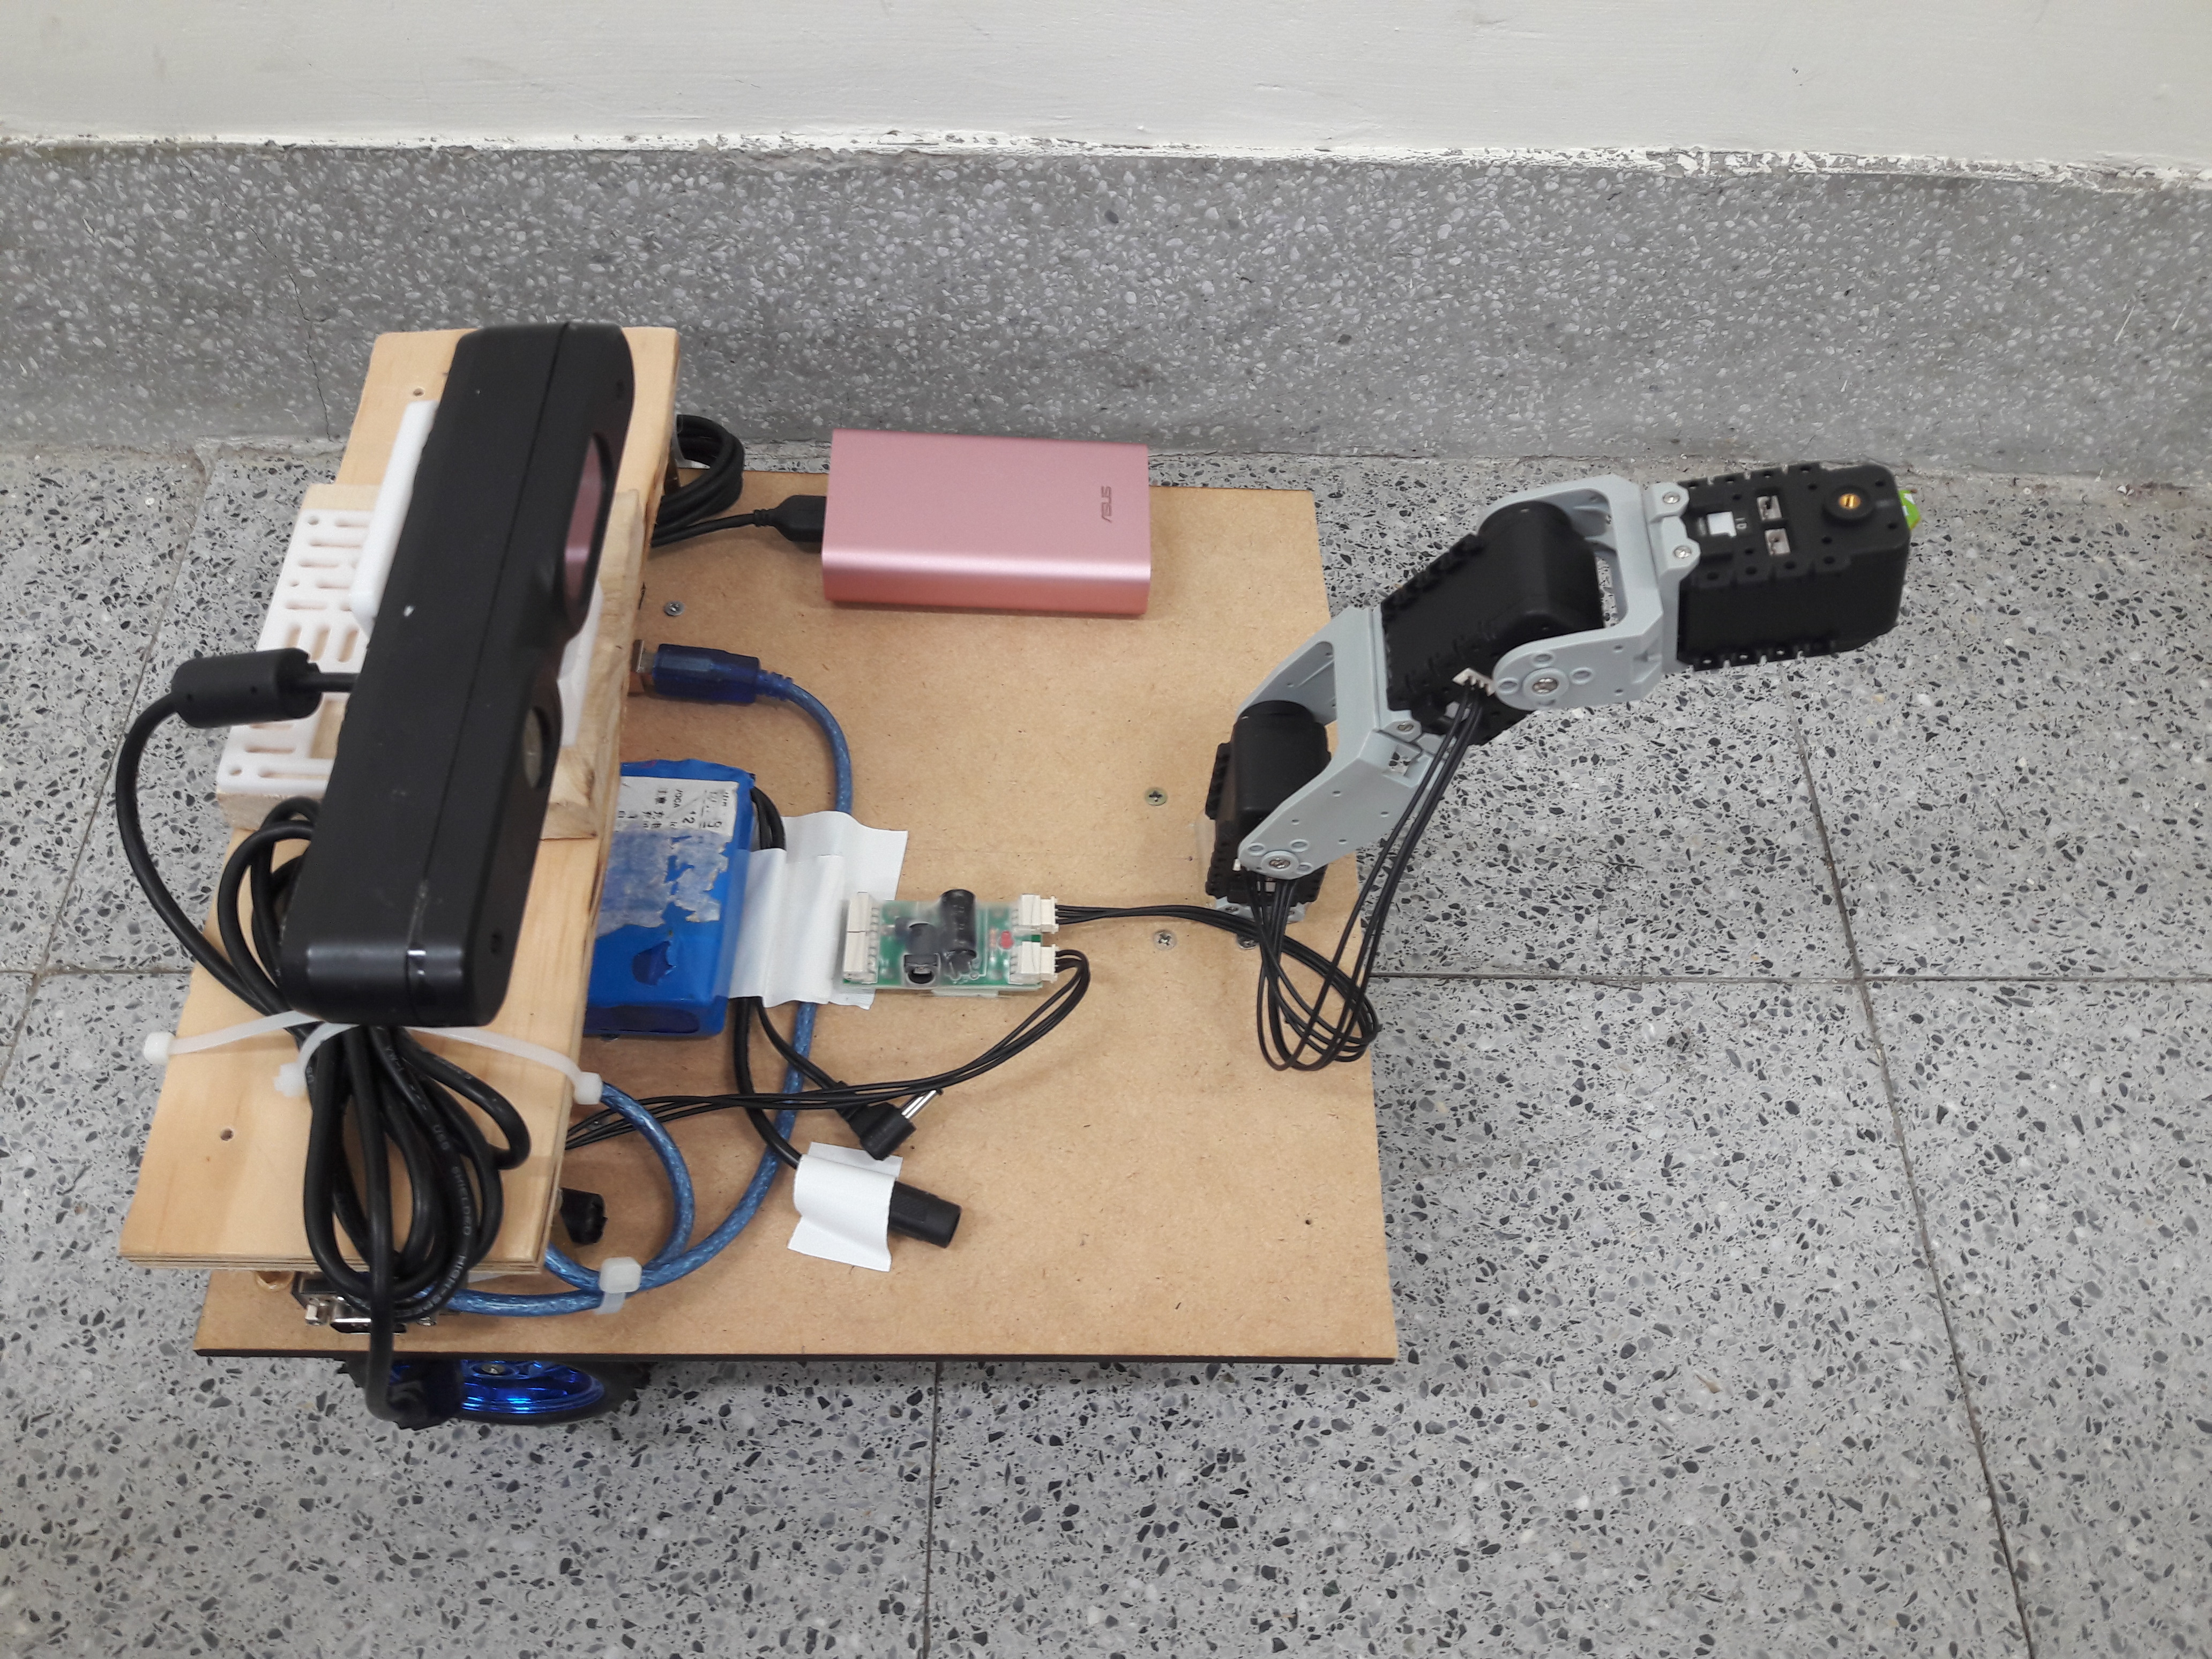
\includegraphics[width=0.7\columnwidth]{robot}
\centering
\caption{MIT2.12 Mobile Manipulator}
 \label{figure:mit212mm}
\end{figure}

\begin{figure}[h]
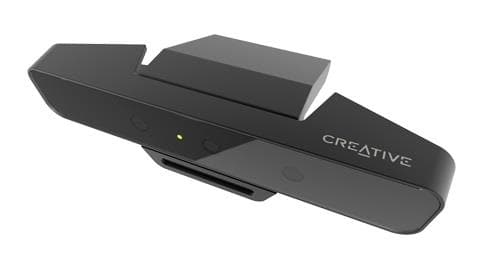
\includegraphics[width=0.7\columnwidth]{RealSense_Camera_SR300_SPL}
\centering
\caption{Intel Realsense SR300}
 \label{figure:sr300}
\end{figure}

